\section{RESULTS AND DISCUSSION}\label{sec:results-and-discussion}
The results illustrated in this section focuses on three scenarios on which Africa's internet topology was simulated. During simulation, link delay which in this project we considered it as the minimum round trip time(RTT) was recorded for each source ASN - destination ASN pair for comparison and evaluation purposes to evaluate which scenario is the best African ISPs can peer at African IXPs. The three scenarios are: pre-simulation scenario where there is no IXP present in the topology, a scenario where one central IXP was added to the topology and a scenario where five regional IXPs were added to the topology. 
 \begin{figure*}
  
    \begin{center}
        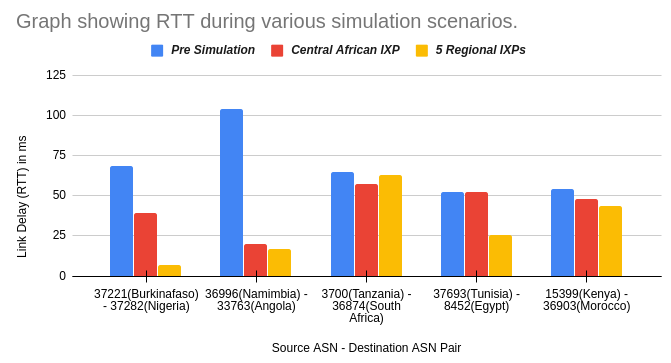
\includegraphics[width=1\linewidth]{sections/pictures-diagrams/graph22.png}
    \end{center}
    \caption{Graph showing RTT during various simulation scenarios.}
    \label{figure:state}
\end{figure*}
Five source ASN - destination ASN pairs were used as tabulated in Table 1. These pairs were chosen to represent the intra-continental Africa internet traffic traversing different regions across the continent. These pairs are namely: 37221(Burkinafaso) - 37282(Nigeria) representing internet traffic originating from ASN 37221 in Burkina Faso to ASN 37282 in Nigeria, 36996(Namimbia) - 33763(Angola) representing internet traffic originating from ASN 36996 in Namimbia to ASN 33763 in Angola, 3700(Tanzania) - 36874(South Africa) representing internet traffic originating from ASN 3700 in Tanzania to ASN 36874 in South Africa, 37693(Tunisia) - 8452(Egypt) representing internet traffic originating from ASN 37693 in Tunisia to ASN 8452 in Egypt and 15399(Kenya) - 36903(Morocco) representing internet traffic originating from ASN 15399 in Kenya to ASN 36903 in Morocco.

 \subsection{Scenarios}
 \subsubsection{Pre-Simulation}
 During this scenario, the topology had no IXP as shown in Figure 7 in the appendix. The scenario is called pre-simulation as it is the initial state of topology where initial measurements of the link delays are recorded for each source ASN - destination ASN. The readings recorded from this phase depicts the real link delays between the source ASN and the destination ASN. These reading are important as they form the base cases to discuss and compare how the link delay will be affected when other scenarios are tested. The results obtained from the pre-simulation phase are tabulated in Table 1. 
 
 \subsubsection{Simulating with a central African IXP}
In this scenario, a central African IXP was added to the topology. The IXP node was added in DRC which is in central Africa. We added the central IXP node in DRC since DRC is in Central Africa and central from all regions in Africa. After adding the IXP node, all source ASN and destination ASNs were connected to the newly introduced IXP. This can be seen well in Figure 13 in the appendix. After all connection had been added, traffic was simulated again to see the change of link delays. The results obtained are tabulated in Table 1.   
  
 \subsubsection{Simulating with 5 regional IXPs}
 In this scenario, 5 regional African IXP were added to the topology. Regional IXPs were added in Algeria for North Africa region, Ghana for West Africa region, Uganda for East Africa and Botswana for the Southern Africa region. These countries are regarded to be central amongst their respective regions. The IXP node that was added in DRC remained as it represented the Central Africa region. After adding the regional IXP nodes, all source ASN and destination ASNs were connected to their respective regional IXPs and all regional IXPs were finally connected to the central IXP node. This can be seen well in Figure 14 in the appendix. After all connections had been added, traffic was simulated again to see the change of link delays. The results obtained are tabulated in Table 1.

 \begin{table}[htp]
   \centering
     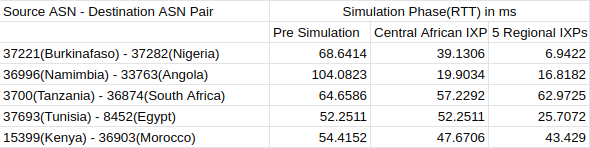
\includegraphics[width=8.5cm]{sections/pictures-diagrams/rttfigures.png}
   \caption{Table showing the RTT of different source ASN - destination ASN Pair when simulated in three scenarios .}
    \label{figure:galaxy}
\end{table}

\subsection{Discussion on the results}
From the graph shown in Figure 5, with the introduction of central African IXP, the link delay of each source ASN - destination ASN decreased by more than 50\% except for the 37639 ASN in Tunisia and 8452 ASN in Egypt. The most significant decrease is the 36696 ASN - 33753 pair due to their close proximity with DRC. The link delays for 37693 ASN - 8452 ASN pair did not decrease due to their presence in North Africa which is quite far from DRC. This scenario shows that, if African ISPs could peer at central Africa IXP located in Central Africa, only internet performance in the South, East, Central and some parts of West Africa Africa will improve. The internet performance in North Africa will still remain the same. Most of the West Africa ISPs peers at IXPs located in France and if they peer at central African IXP, inter-regional internet performance may improve as shown by the ASN 37221 (Burkinafaso) - ASN 37282 (Nigeria).

In the scenario where five regional IXPs were introduced in the topology, the regional internet performance improved highly as the link delay decreased by more than 75\% but also the inter-regional internet performance improved as the link delay dropped by 20\%. The inter-regional traffic is represented by traffic originating from 15399 ASN in Kenya to 36903 ASN in Morocco and 3700 ASN in Tanzania to 36874 ASN in South Africa.

This shows that African ISPs should peer at regional IXPs to ensure that regional internet performance is good and the regional IXPs should be connected to a central IXP to ensure that inter-regional internet performance also improves.  
